\chapter{OLAY MÜDAHALE VE ADLİ BİLİŞİM}

\section*{Giriş}
Olay müdahale ve adli bilişim (DFIR - Digital Forensics and Incident Response), siber güvenlik olaylarının tespiti, analizi, müdahalesi ve sonrasında delil toplama süreçlerini kapsayan kritik bir disiplindir. Bu bölümde, modern DFIR metodolojileri, araçları ve teknikleri detaylı olarak ele alınacaktır.



\section{Olay Müdahale Temelleri ve Metodolojiler}

\begin{figure}[H]
    \centering
    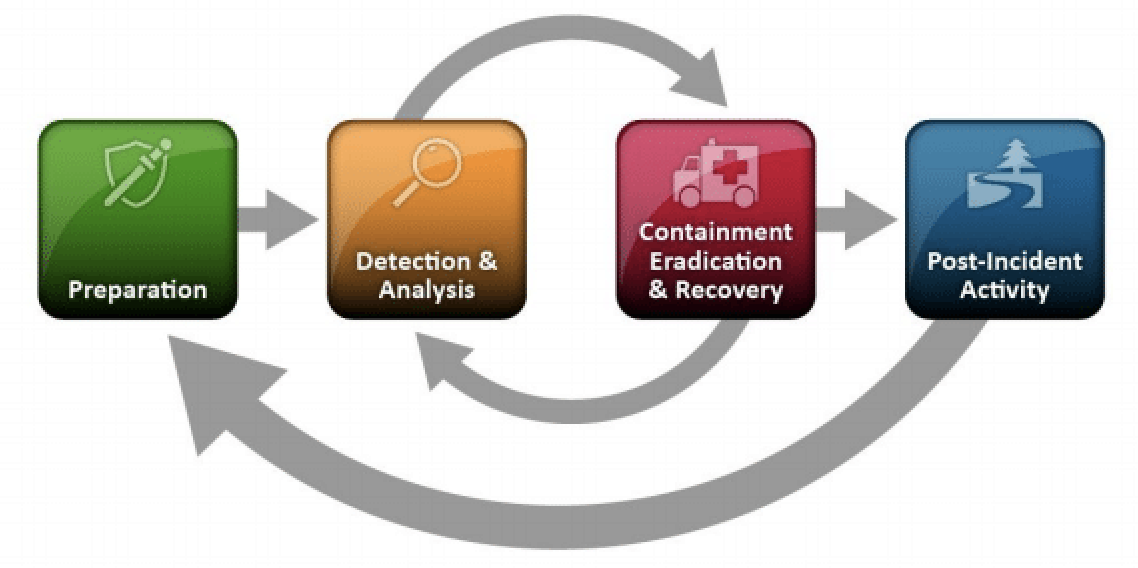
\includegraphics[width=0.8\textwidth]{img/IR.png}
    \caption{Olay Müdahale (Incident Response) Süreci ve Metodolojileri}
    \label{fig:incident-response}
\end{figure}

\begin{figure}[H]
    \centering
    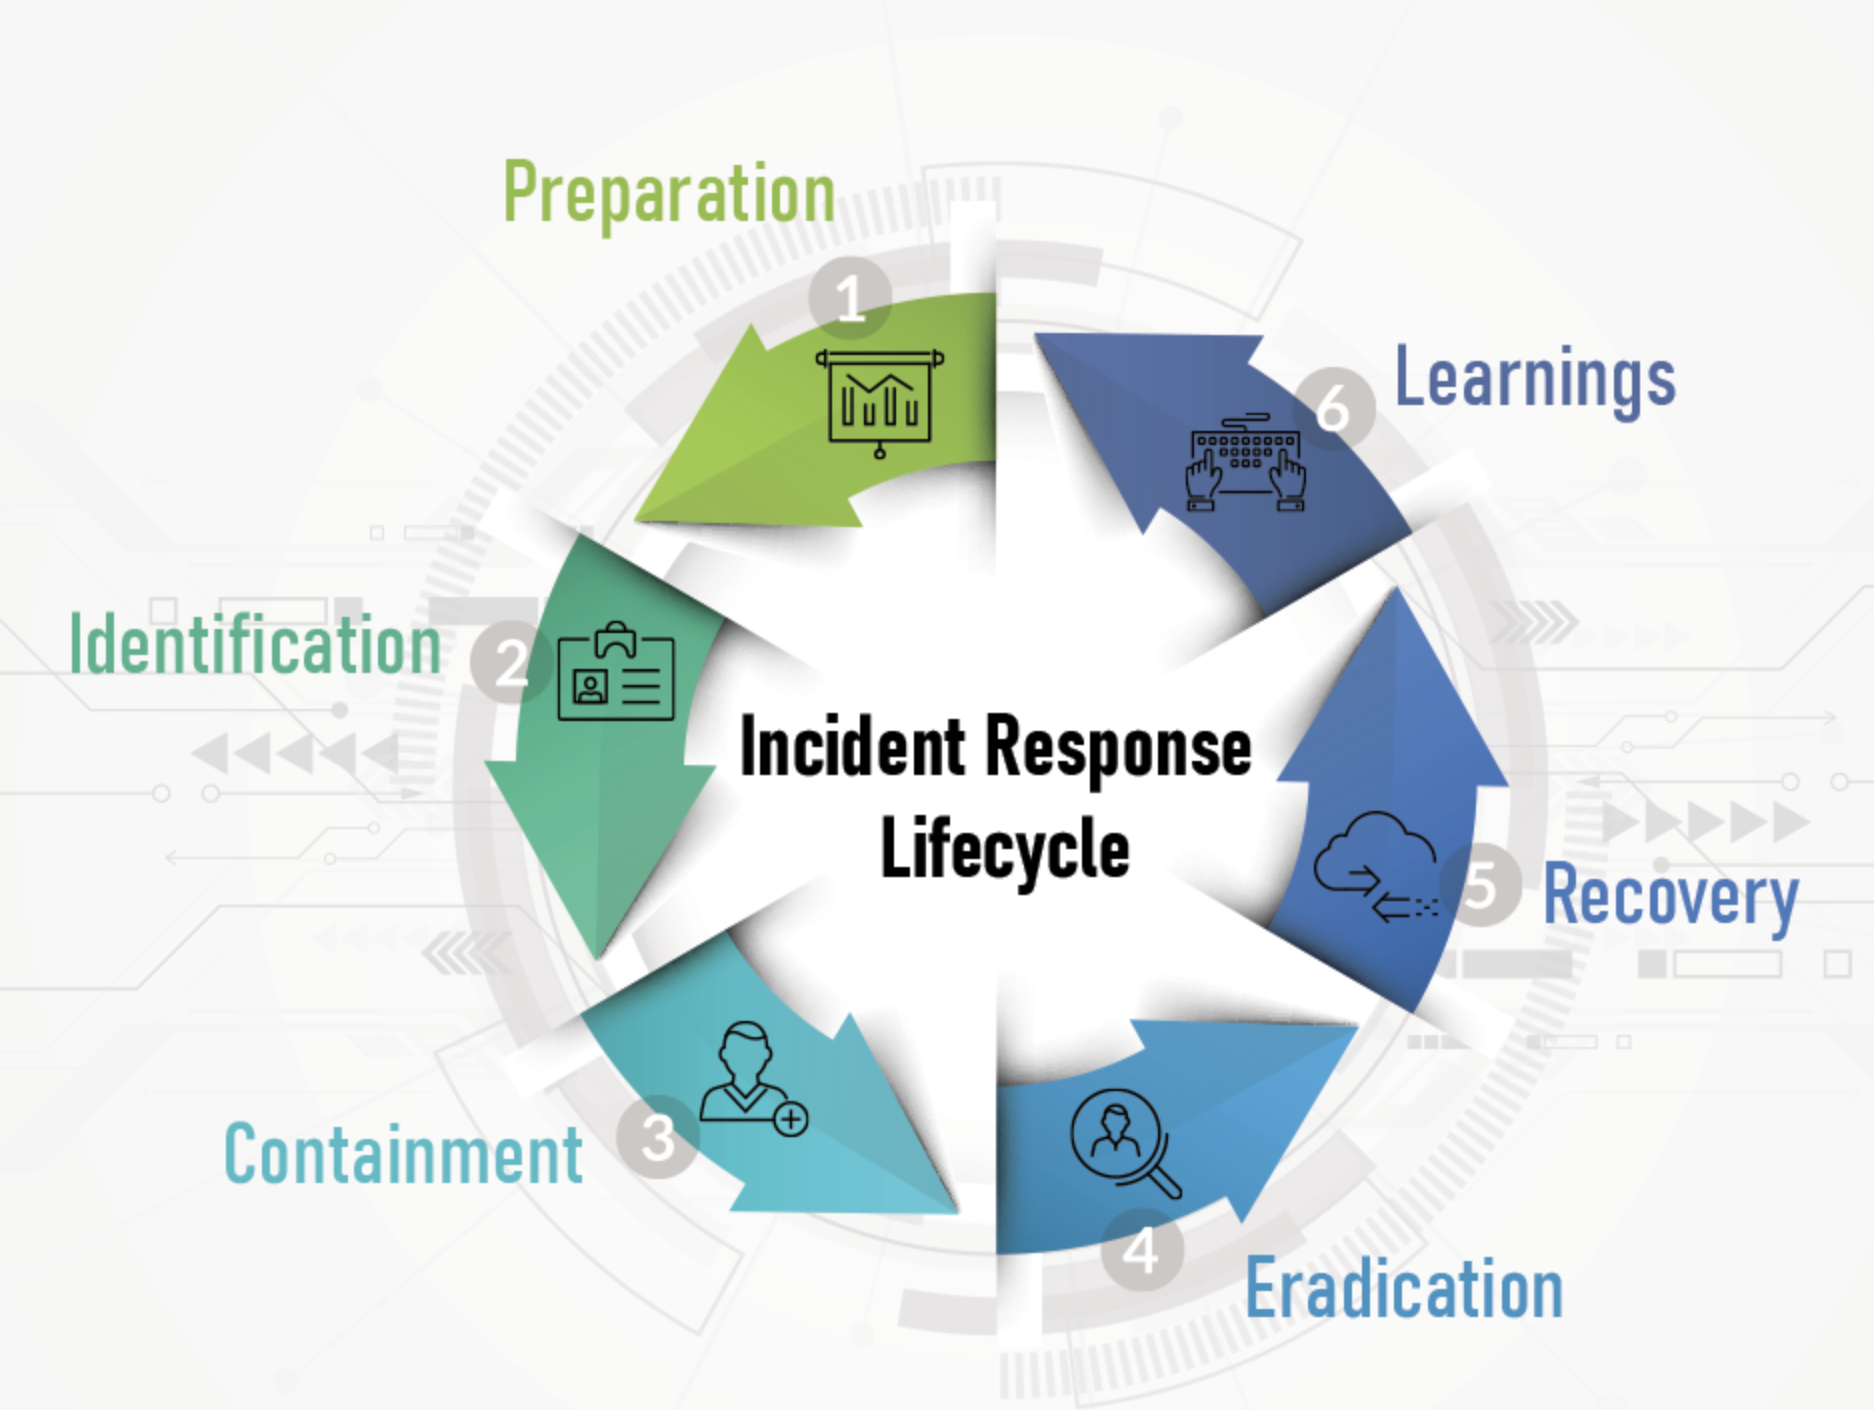
\includegraphics[width=0.8\textwidth]{img/IR_lifecycle.png}
    \caption{Olay Müdahale Yaşam Döngüsü ve Süreç Adımları}
    \label{fig:ir-lifecycle}
\end{figure}



\subsection{Gelişmiş Saldırı Göstergeleri ve Tehdit Avlama}

\subsection{DFIR Metodolojileri: SANS ve NIST Karşılaştırması}

Olay müdahale ve dijital adli bilişim (DFIR) alanında en yaygın kullanılan iki metodoloji, SANS ve NIST'in geliştirdiği çerçevelerdir. Bu metodolojiler, organizasyonların siber olaylara karşı hazırlıklı olmasını ve etkili müdahale etmesini sağlar.

\begin{figure}[H]
    \centering
    
\includegraphics[width=0.7\textwidth]{img/sans-dfir.png}
    \caption{SANS DFIR Metodolojisi ve Süreç Adımları}      
    \label{fig:sans-dfir}
\end{figure}\subsubsection{SANS DFIR Metodolojisi}

SANS, dünya genelinde en çok kullanılan altı adımlı Olay Müdahale (Incident Response) sürecini önerir:

\begin{enumerate}
    \item \textbf{Hazırlık (Preparation):}
    \begin{itemize}
        \item Politika, olay müdahale planı ve araçların oluşturulması
        \item İletişim kanallarının belirlenmesi
        \item Personel eğitimlerinin tamamlanması
    \end{itemize}

    \item \textbf{Tespit (Identification):}
    \begin{itemize}
        \item Olası güvenlik olaylarının belirlenmesi
        \item Uyarılar ve logların analizi
        \item Tehdit istihbaratı ve anomali tespiti
    \end{itemize}

    \item \textbf{Sınırlama (Containment):}
    \begin{itemize}
        \item Kısa vadeli: Etkilenen sistemlerin izolasyonu
        \item Uzun vadeli: Yamalar, güvenlik duvarı kuralları ve ağ segmentasyonu
    \end{itemize}

    \item \textbf{Ortadan Kaldırma (Eradication):}
    \begin{itemize}
        \item Zararlı yazılımın temizlenmesi
        \item Açıklıkların kapatılması
        \item Saldırganın kalıcılığının yok edilmesi
    \end{itemize}

    \item \textbf{Kurtarma (Recovery):}
    \begin{itemize}
        \item Sistemlerin geri yüklenmesi
        \item Bütünlüğün doğrulanması
        \item Normal işleyişe dönüş
    \end{itemize}

    \item \textbf{Dersler (Lessons Learned):}
    \begin{itemize}
        \item Olay sonrası değerlendirme ve raporlama
        \item Kök neden analizi
        \item Savunma mekanizmalarının geliştirilmesi
    \end{itemize}
\end{enumerate}

\subsubsection{NIST DFIR Metodolojisi}

NIST SP 800-61 (Bilgisayar Güvenliği Olay Müdahale Rehberi) dokümanında tanımlanan süreç dört ana aşamadan oluşur:

\begin{enumerate}
    \item \textbf{Hazırlık (Preparation):}
    \begin{itemize}
        \item Politika belirleme ve personel eğitimi
        \item İletişim kanallarının tanımlanması
        \item Tespit araçlarının kurulması
    \end{itemize}

    \item \textbf{Tespit ve Analiz (Detection \& Analysis):}
    \begin{itemize}
        \item Güvenlik uyarıları ve logların izlenmesi
        \item Olayın kapsamı ve türünün belirlenmesi
        \item Ciddiyet sınıflandırması ve önceliklendirme
    \end{itemize}

    \item \textbf{Sınırlama, Ortadan Kaldırma ve Kurtarma:}
    \begin{itemize}
        \item Olayın etkisinin durdurulması
        \item Kök nedenin ortadan kaldırılması
        \item Sistemlerin geri yüklenmesi ve izlenmesi
    \end{itemize}

    \item \textbf{Olay Sonrası Faaliyetler:}
    \begin{itemize}
        \item Alınan derslerin dokümantasyonu
        \item Olay detaylarının belgelenmesi
        \item IR planı ve güvenlik mimarisinin güncellenmesi
    \end{itemize}
\end{enumerate}

\subsubsection{DFIR Metodolojileri}

\begin{table}[ht]
\centering
\begin{tabular}{|l|l|l|}
\hline
\textbf{Kriter} & \textbf{SANS} & \textbf{NIST} \\
\hline
Köken & Eğitim \& sertifikasyon kurumu & ABD federal standart kurumu \\
\hline
Odak & Pratik, uygulayıcı odaklı & Stratejik, politika \& uyumluluk odaklı \\
\hline
DFIR Modeli & 6 adım & 4 adım \\
\hline
Güçlü Yanı & Operasyonel, sahada uygulanabilir & Standartlaştırılmış, politika uyumlu \\
\hline
Kullanım & SOC/IR ekipleri & ABD kamu sektörü \& uyumluluk \\
\hline
\end{tabular}
\caption{DFIR Metodolojileri Karşılaştırması}
\end{table}

Kurumlar genellikle bu iki metodolojinin birleşimini kullanır:
\begin{itemize}
    \item NIST → Politika ve standartlar için
    \item SANS → Operasyonel uygulama için
\end{itemize}

\begin{itemize}
    \item \textbf{Tehdit Avlama Metodolojileri:}
    \begin{itemize}
        \item \textbf{Hipotez Bazlı Avlama:} Örnek: "Sistemde PowerShell Empire kullanıldığına dair göstergeler var mı?"
        \item \textbf{İstihbarat Bazlı Avlama:} Bilinen APT gruplarların TTPs'lerine dayalı arama
        \item \textbf{Anomali Bazlı Avlama:} Normal sistem davranışından sapmaların tespiti
    \end{itemize}

    \item \textbf{Gelişmiş IOC'ler:}
    \begin{itemize}
        \item \textbf{YARA Kuralları:} Zararlı yazılım ailelerini tespit etmek için özel imza tanımları
        \item \textbf{SIGMA Kuralları:} SIEM sistemleri için standartlaştırılmış log analiz kuralları
        \item \textbf{Snort/Suricata Kuralları:} Ağ trafiğinde zararlı aktivite tespiti için kullanılan kurallar
    \end{itemize}

    \item \textbf{Hazırlık (Preparation):} Olayların meydana gelme olasılığını azaltmak için proaktif önlemlerin alındığı aşamadır. Bu aşama, güvenlik açıklarının belirlenmesini ve azaltılmasını, güvenlik politikaları ile prosedürlerinin tanımlanmasını ve bilişim varlıklarının risk analizine göre önceliklendirilmesini içerir. Etkili bir hazırlık için, bir Bilgisayar Güvenlik Olay Müdahale Ekibinin (CSIRT) oluşturulması, iç ve dış paydaşlarla iletişim kanallarının kurulması ve düzenli masa başı (tabletop) tatbikatlarının yapılması hayati önem taşır.

    \item \textbf{Pratik Senaryo - Hazırlık Aşaması Tatbikatı:}
    \begin{itemize}
        \item Bir fidye yazılımı saldırısı için masa başı tatbikatı ele alınabilir. Senaryoda, bir çalışanın e-posta yoluyla fidye yazılımını sisteme bulaştırdığı varsayılır. Olay müdahale ekibi, bu simülasyon sırasında rolleri ve sorumlulukları üzerinden aşağıdaki adımları tartışır:
        \begin{itemize}
            \item Hangi varlıkların (sunucular, veritabanları) öncelikli olarak izole edilmesi gerektiği
            \item İş sürekliliğini sağlamak için hangi alternatif sistemlerin devreye alınacağı
            \item Üst yönetim, hukuk departmanı ve halkla ilişkiler ile hangi iletişim kanallarının kullanılacağı
            \item Verilerin geri yüklenmesi için yedekleme altyapısının test edilmesi ve doğrulanması
        \end{itemize}
    \end{itemize}

\begin{itemize}
    \item \textbf{Tespit ve Analiz (Detection \& Analysis):} Bu aşama, güvenlik olaylarının sürekli izlenmesini ve toplanan verilerin analiz edilmesini içerir. Amaç, şüpheli etkinlikleri gerçek bir siber olaydan ayırt etmektir. Olayın doğası, kapsamı, kökeni ve potansiyel etkisi bu aşamada belirlenir.

    \item \textbf{Sınırlama, Yok Etme ve Kurtarma (Containment, Eradication \& Recovery):} Tespit ve analiz aşamasının ardından, saldırının yayılmasını durdurmak ve zararı en aza indirmek için harekete geçilir. Bu, tehdidin sistemden tamamen temizlenmesini ve iş operasyonlarının normal durumuna geri döndürülmesini kapsar.
\end{itemize}

\subsection{MITRE ATT\&CK Çerçevesi ve Saldırı Tespit Stratejileri}

MITRE ATT\&CK, saldırganların kullandığı taktik ve teknikleri kategorize eden kapsamlı bir bilgi tabanıdır. Bu çerçeve, olay müdahale ve adli bilişim süreçlerinde saldırıların analizi ve savunma stratejilerinin geliştirilmesi için kullanılır.

\begin{itemize}
    \item \textbf{Olay Sonrası Faaliyetler (Post-Incident Activity):} Olay müdahalesinin tamamlanmasından sonra gerçekleştirilen bu aşama, yaşanan olaydan dersler çıkarmayı ve elde edilen bilgileri gelecekteki güvenlik tedbirlerini güçlendirmek için kullanmayı hedefler. Bu süreç, organizasyonun savunma duruşunu sürekli olarak iyileştirme amacını taşır.
\end{itemize}

\subsection{ATT\&CK Matrisi Kullanımı}

\begin{itemize}
    \item \textbf{Taktikler ve Teknikler:}
    \begin{itemize}
        \item \textbf{Başlangıç Erişimi (Initial Access):} Oltalama e-postaları, güvenlik açıklarının istismarı
        \item \textbf{Yetki Yükseltme (Privilege Escalation):} Sistem zafiyetleri, token çalma
        \item \textbf{Yanal Hareket (Lateral Movement):} Pass-the-hash, uzak masaüstü protokolü
        \item \textbf{Veri Hırsızlığı (Exfiltration):} Alternatif protokoller, steganografi
    \end{itemize}

\subsection{Bilgisayar Güvenlik Olay Müdahale Ekibi (CSIRT) Yapısı}

CSIRT, bir organizasyondaki siber güvenlik olaylarını yönetmekle görevli, disiplinler arası ve özel bir ekiptir. Bu ekibin temel amacı, hasarı en aza indirmek ve iş sürekliliğini sağlamaktır. Etkili bir CSIRT operasyonu, sadece teknik uzmanlık değil, aynı zamanda idari ve yasal yetkinlikler de gerektirir.

\begin{itemize}
    \item \textbf{Roller ve Sorumluluklar:} CSIRT, olay yönetimi sürecinin tüm yaşam döngüsünü (hazırlık, tespit, analiz, sınırlama, yok etme, kurtarma ve olay sonrası inceleme) yönetir. Ekip üyeleri, altyapı, işletim sistemleri ve uygulamalar hakkında derinlemesine bilgiye sahip olmalı; etik hacking, bulut güvenliği ve log analizi gibi alanlarda uzmanlık sergilemelidir.

    \item \textbf{Çapraz Fonksiyonel Yapı:} Bir CSIRT, yalnızca teknik uzmanlardan oluşmamalıdır. Hukuk, iletişim, insan kaynakları ve kritik iş birimi yöneticileri gibi farklı departmanlardan temsilcileri içermelidir. Bu çok disiplinli yapı, bir siber saldırının teknik boyutlarının yanı sıra yasal ve itibari sonuçlarının da bütüncül bir yaklaşımla ele alınmasını sağlar. Yönetimden destek ve onay almak, bu ekibin etkin bir şekilde çalışabilmesi için başlangıçta atılması gereken en önemli adımlardan biridir.
\end{itemize}

\subsection{Zararlı Yazılım Analiz Teknikleri}

Modern zararlı yazılımlar, tespit edilmemek için gelişmiş teknikler kullanır. Bu yazılımları analiz etmek için hem statik hem de dinamik analiz teknikleri kullanılır.

\begin{itemize}
    \item \textbf{Statik Analiz:}
    \begin{itemize}
        \item Dosya imzaları ve hash değerleri kontrolü
        \item PE başlık analizi ve bağımlılık incelemesi
        \item Dizi analizi ve şüpheli API çağrılarının tespiti
        \item Yürütülebilir dosya yapısının incelenmesi
    \end{itemize}
\end{itemize}

\subsection{Olay Sınıflandırma, Önceliklendirme ve Ciddiyet Değerlendirmesi}

Olay müdahale sürecinin ilk adımlarından biri, bir olayın ciddiyetini ve potansiyel etkisini değerlendiren "triyaj" sürecidir. Bu aşama, kısıtlı kaynakların en kritik olaylara yönlendirilmesini sağlar ve yanlış pozitif alarmların filtrelenmesine yardımcı olur. Olaylar, saldırı türlerine göre farklı öncelik seviyelerine ayrılır. Örneğin:

\begin{itemize}
    \item \textbf{Keşif ve Araştırma (Probe):} Saldırganın bilgi toplamaya çalıştığı düşük öncelikli olaylar.
    \item \textbf{İstismar ve Kurulum (Exploit \& Installation):} Bir zafiyetin sömürülmesi veya kötü amaçlı yazılımın sisteme yerleştirilmesi girişimi. Bu orta/yüksek öncelikli bir olaydır.
    \item \textbf{Sistemin Ele Geçirilmesi (System Compromise):} Saldırganın sisteme tam erişim sağladığı, en yüksek öncelikli olaydır.
\end{itemize}

\textbf{Pratik Senaryo - Alarm Triyajı:}

Bir SIEM sistemi, aynı IP adresinden 30 saniye içinde 6 başarısız oturum açma girişimi için bir alarm üretir. Bir siber güvenlik analisti bu durumu şu adımlarla yönetir:

\begin{enumerate}
    \item \textbf{Gözden Geçirme:} Analist, alarmı inceler ve benzer olayların geçmişte yaşanıp yaşanmadığını, bu IP adresinin bilinen bir zafiyet tarayıcısına ait olup olmadığını kontrol eder.
    \item \textbf{Sınıflandırma:} Etkinlik, "Brute Force Saldırı Girişimi" olarak sınıflandırılır.
    \item \textbf{Öncelik Belirleme:} Bu bir girişimi temsil ettiği ve henüz sisteme sızma gerçekleşmediği için öncelik seviyesi "Orta" olarak belirlenir.
    \item \textbf{Eskalasyon ve Aksiyon:} Analist, eğer birden fazla IP'den benzer aktiviteler geliyorsa durumu daha ileri analiz için Seviye 2 analiste bildirir ve ilgili IP adresinin güvenlik duvarı üzerinden geçici olarak engellenmesi için bir kural başlatır.
\end{enumerate}

\begin{itemize}
    \item \textbf{Dinamik Analiz:}
    \begin{itemize}
        \item Sanal makine veya sandbox ortamında çalıştırma
        \item Sistem çağrıları ve ağ trafiğinin izlenmesi
        \item Bellek değişikliklerinin analizi
        \item Anti-analiz tekniklerinin tespiti ve bypass edilmesi
    \end{itemize}

    \item \textbf{Davranışsal Analiz:}
    \begin{itemize}
        \item Dosya sistemi aktivitelerinin izlenmesi
        \item Registry değişikliklerinin takibi
        \item Ağ bağlantılarının analizi
        \item Süreç ve servis değişikliklerinin kontrolü
    \end{itemize}
\end{itemize}

\subsection{İletişim Planları ve Paydaş Yönetimi}

Etkin bir olay müdahale planının en önemli bileşenlerinden biri, iç ve dış paydaşlarla nasıl iletişim kurulacağını belirleyen önceden hazırlanmış bir iletişim planıdır. Bu plan, olayın teknik yönlerinin yanı sıra organizasyonun itibarı ve paydaş güveni üzerindeki potansiyel etkilerini yönetmek için tasarlanmıştır.

\begin{itemize}
    \item \textbf{Kritik Paydaşlar:}
    \begin{itemize}
        \item \textbf{İç Paydaşlar:} Üst yönetim, hukuk departmanı, halkla ilişkiler, insan kaynakları ve kritik iş birimi yöneticileri.
        \item \textbf{Dış Paydaşlar:} Yasal ve düzenleyici kurumlar (örneğin Kişisel Verileri Koruma Kurumu), kolluk kuvvetleri, müşteriler, tedarikçiler ve basın.
    \end{itemize}
\end{itemize}

\textbf{Pratik Senaryo - İletişim Akışı:}

Bir veri sızıntısı durumunda iletişim süreci aşağıdaki gibi işleyebilir:

\begin{enumerate}
    \item \textbf{Dahili Bildirim:} CSIRT lideri, veri sızıntısının tespitini hemen üst yönetime ve ilgili iç paydaşlara bildirir. Teknik ekip olayın kapsamını belirlerken, halkla ilişkiler ve hukuk departmanları potansiyel yasal ve kamuoyu yansımaları için hazırlık yapar.
    \item \textbf{Hukuki Bildirim:} Hukuk departmanı, veri sızıntısının yürürlükteki yasalara (ör. KVKK) göre bildirim gerektirip gerektirmediğini değerlendirir. Yasal bildirim süresine uyarak, ilgili düzenleyici kurumlara "derhal" bildirimde bulunulur.
    \item \textbf{Dış Paydaş İletişimi:} İletişim planına uygun olarak, halkla ilişkiler ekibi, durumu net, şeffaf ve abartısız bir dille açıklayan bir basın açıklaması veya müşteri bildirimi hazırlar. Bu açıklama, olayın doğasını, alınan önlemleri ve gelecekteki adımları içerir ve organizasyonun itibarını korumaya yardımcı olur.
\end{enumerate}

\subsection{SOAR (Security Orchestration, Automation and Response)}

SOAR sistemleri, olay müdahale süreçlerini otomatikleştirerek yanıt süresini kısaltır ve insan hatasını azaltır.

\begin{itemize}
    \item \textbf{Otomatik Müdahale Playbook'ları:}
    \begin{itemize}
        \item \textbf{Oltalama E-posta Müdahalesi:}
        \begin{enumerate}
            \item E-postanın otomatik karantinaya alınması
            \item Benzer e-postaların tüm posta kutularında aranması
            \item Şüpheli URL'lerin otomatik engellenmesi
            \item Etkilenen kullanıcıların bilgilendirilmesi
        \end{enumerate}
        \item \textbf{Zararlı Yazılım Müdahalesi:}
        \begin{enumerate}
            \item Etkilenen sistemin otomatik izolasyonu
            \item Zararlı yazılımın karantinaya alınması
            \item Sistem geri yükleme noktası oluşturulması
            \item IOC'lerin SIEM'e otomatik eklenmesi
        \end{enumerate}
    \end{itemize}
\end{itemize}

\begin{itemize}
    \item \textbf{Kolluk Kuvvetleri ile İşbirliği:} Özellikle ciddi siber suçlarda, Türkiye'deki Ulusal Siber Olaylara Müdahale Merkezi (USOM) ve Siber Olaylara Müdahale Ekipleri (SOME) gibi ulusal otoritelerle koordinasyon sağlanması zorunludur.

    \item \textbf{Adli Geçerlilik:} Bir olay sırasında toplanan delillerin mahkemede geçerli sayılması için "gözetim zinciri" (Chain of Custody) olarak bilinen bir prosedürün titizlikle uygulanması gerekir. Bu prosedür, delilin toplanmasından mahkemeye sunulmasına kadar geçen her adımın belgelenmesini, delil bütünlüğünün (hash değerleri ile) korunmasını ve yetkisiz erişime karşı güvenli bir şekilde saklanmasını gerektirir.
\end{itemize}

Olay müdahale süreci, sadece teknik bir problem çözme döngüsü değil, aynı zamanda bütüncül bir kriz yönetimi sürecidir. Bu durum, BT ve güvenlik ekiplerinin, hukuk, iletişim ve üst yönetim gibi diğer departmanlarla sürekli ve entegre bir işbirliği içinde olması gerektiği anlamına gelir. Bu işbirliğinin eksikliği, teknik olarak başarılı bir müdahalenin bile yasal veya itibari bir başarısızlıkla sonuçlanmasına neden olabilir.

\section{Dijital Adli Bilişim Süreçleri}

\subsection{Güvenlik Olayı İzleme ve Alarm Korelasyonu}

Güvenlik Olayı ve Bilgi Yönetimi (SIEM) sistemleri, bir organizasyonun ağındaki çeşitli kaynaklardan gelen günlük (log) verilerini toplayarak şüpheli olayları tespit eder. Alarm korelasyonu, bu sistemlerin sağladığı en önemli işlevlerden biridir. Tek bir olaydan kaynaklanan yüzlerce gereksiz alarmın ("alarm gürültüsü") filtrelenmesini ve bu karmaşanın gerçek tehditlerin gizlenmesine yol açmasının önlenmesini sağlar.

\begin{itemize}
    \item \textbf{API Entegrasyonları:}
    \begin{itemize}
        \item Güvenlik duvarı kurallarının otomatik güncellenmesi
        \item EDR sistemleri ile entegrasyon
        \item Tehdit istihbaratı platformları ile veri alışverişi
        \item İş emri sistemleri ile entegrasyon
    \end{itemize}
    
    \item \textbf{Pratik Korelasyon Kural Örnekleri:}
    \begin{itemize}
        \item \textbf{Brute Force Saldırı Tespiti:} Bir SIEM sistemi, "aynı IP adresinden 30 saniye içinde 6'dan fazla başarısız oturum açma girişimi olursa alarm üret" kuralı ile deneme yanılma saldırılarını otomatik olarak tespit edebilir.
        \item \textbf{Zararlı Yazılım Kontrolü:} "Endpoint koruma sistemi tarafından zararlı olarak tespit edilen bir IP adresi aynı zamanda kritik bir sunucuya oturum başlatırsa alarm üret" kuralı, saldırganın yanal hareketlerini saptamaya yardımcı olur.
        \item \textbf{Log Kaynağı Davranışı Tespiti:} Saldırganlar, tespit edilmekten kaçınmak için log kaynaklarını devre dışı bırakabilirler. Bu duruma karşı "bir uç sistem 1 saatten uzun süre log göndermemişse alarm üret" gibi kurallar yazılabilir.
    \end{itemize}
\end{itemize}

\subsection{Veri Bilimi ve Yapay Zeka Teknikleri}

Modern DFIR süreçleri, büyük veri analizi ve yapay zeka tekniklerinden faydalanır.

\begin{itemize}
    \item \textbf{Makine Öğrenmesi Uygulamaları:}
    \begin{itemize}
        \item \textbf{Anormal Davranış Tespiti:} Kullanıcı davranış analizi (UBA), ağ trafiği anomali tespiti, dosya sistemi aktivite analizi
        \item \textbf{Tehdit İstihbaratı Analizi:} IOC kümeleme ve sınıflandırma, saldırı kampanyası ilişkilendirme, tehdit aktörü profilleme
    \end{itemize}

    \item \textbf{Derin Öğrenme Uygulamaları:} Zararlı yazılım sınıflandırma, şifrelenmiş trafikte anormal davranış tespiti, sıfırıncı gün saldırılarının tespiti
\end{itemize}

\subsection{İlk Müdahale ve Triyaj Prosedürleri}

Olay tespiti yapıldıktan sonraki ilk ve en kritik adım, olayın kapsamını ve önceliğini belirleyen triyaj prosedürleridir. Bu süreç, bir olayın yanlış pozitif mi, yoksa gerçek bir güvenlik ihlali mi olduğunu hızla belirlemeye ve doğru müdahale ekibini atamaya odaklanır.

\begin{itemize}
    \item \textbf{Triyaj Süreci Adımları:}
    \begin{enumerate}
        \item \textbf{Gözden Geçirme:} Seviye 1 analist, SIEM'den gelen alarmı inceler ve bilinen bir güvenlik tarama aracı veya yazılım güncellemesi gibi meşru bir aktivite olup olmadığını kontrol eder.
        \item \textbf{Doğrulama:} Eğer şüphe devam ederse, analist ilgili log kayıtlarını (güvenlik duvarı, uygulama, sistem logları) ve ağ trafiğini inceleyerek olayın gerçek bir saldırı olduğunu doğrular.
        \item \textbf{Sınıflandırma ve Önceliklendirme:} Olay, önceden tanımlanmış kategorilere (ör. oltalama, fidye yazılımı) ve risk matrisine göre (Etki x Ciddiyet) sınıflandırılır ve önceliklendirilir.
        \item \textbf{Eskalasyon:} Olayın ciddiyetine göre, sorumlu yöneticilere ve daha ileri düzeyde teknik yetkinliğe sahip Seviye 2 analistlere bildirimde bulunulur.
    \end{enumerate}
\end{itemize}

\subsection{Delil Toplama ve Gözetim Zinciri Yönetimi}

Dijital delillerin toplanması, adli bilişim sürecinin temelini oluşturur. Bu delillerin, hukuki süreçlerde geçerli sayılabilmesi için değiştirilmediğinden, silinmediğinden ve manipüle edilmediğinden emin olunması gereklidir. Delilin bütünlüğünü korumak için, toplama işlemi sırasında dosyanın "hash" değeri (parmak izi) hesaplanır ve herhangi bir değişiklikte bu değerin değişeceği kabul edilir.

\begin{itemize}
    \item \textbf{Gözetim Zinciri (Chain of Custody):} Bu kavram, delilin olay yerinden toplanmasından mahkemeye sunulmasına kadar geçen süredeki tüm adımların titizlikle belgelenmesini ifade eder. Bu zincir, delilin doğru bir şekilde işlendiğini ve manipüle edilmediğini kanıtlayarak hukuki geçerliliğini sağlar.
\end{itemize}

\textbf{Delil Gözetim Zinciri Formu Örneği}

\begin{tabular}{|l|l|l|l|l|l|l|l|}
\hline
Delil Numarası & Delil Tanımı & Toplama Tarihi/Saati & Toplama Yeri & Hash Değeri (SHA256) & Toplayan Personel & Taşıma Bilgisi & Saklama Konumu \\
\hline

IR-2024-001-H1 & Sunucu 1'in fiziksel disk imajı & 2024-05-15, 10:00 & Sunucu Odası A & \texttt{e4c8e75...} & Ali Kaya & Sınırlı Erişim Deposu & Depo-1, Kilitli Dolap C \\
\hline
IR-2024-001-R1 & Sunucu 1'in RAM dökümü & 2024-05-15, 10:05 & Sunucu Odası A & \texttt{3a5a7d9...} & Veli Yılmaz & Ali Kaya'ya devir, 10:15 & Depo-1, Kilitli Dolap C \\
\hline
\end{tabular}
\end{itemize}

\subsection{Kök Neden Analizi ve Saldırı Vektörü Belirleme}

Kök Neden Analizi (RCA), bir siber saldırının yalnızca yüzeysel nedenlerini (ör. bir bilgisayarın enfekte olması) değil, aynı zamanda olayın temelinde yatan asıl nedeni bulmayı amaçlayan sistematik bir çözme yöntemidir. Bu analiz, "neden" sorusunu tekrar tekrar sorarak saldırının nasıl gerçekleştiğini ve hangi zafiyetin sömürüldüğünü detaylıca ortaya çıkarır.

\begin{itemize}
    \item \textbf{Pratik Senaryo - RCA Uygulaması ("5 Neden" Tekniği):}
    \begin{itemize}
        \item \textbf{Sorun:} Kurumun web sitesi, bir siber saldırı sonucu erişilemez hale geldi.
        \item \textbf{1. Neden?} Web sitesi neden erişilemez hale geldi? Çünkü saldırgan SQL enjeksiyonuyla veritabanını sildi.
        \item \textbf{2. Neden?} Saldırgan neden veritabanını silebildi? Çünkü web uygulamasının kullanıcı girdileri düzgün bir şekilde filtrelenmiyordu.
        \item \textbf{3. Neden?} Girdiler neden filtrelenmiyordu? Çünkü geliştirme ekibi bu güvenlik zafiyetini göz ardı eden eski bir kütüphane kullanıyordu.
        \item \textbf{4. Neden?} Bu zafiyet neden göz ardı edildi? Çünkü geliştirme yaşam döngüsüne (SDLC) düzenli güvenlik testleri ve kod incelemeleri entegre edilmemişti.
        \item \textbf{Kök Neden:} Yazılım geliştirme süreçlerinde güvenli kodlama politikalarının ve testlerinin olmamasıdır. Bu analiz, yüzeysel bir teknik sorunun (SQL enjeksiyonu) aslında daha derin bir sistemsel politika eksikliğinden kaynaklandığını göstermektedir.
    \end{itemize}
\end{itemize}

\subsection{Zaman Çizelgesi Oluşturma ve Saldırı Rekonstrüksiyonu}

Olayın her aşamasının kronolojik olarak sıralandığı bir zaman çizelgesi, saldırının nasıl başladığını, nasıl yayıldığını ve hangi sistemleri etkilediğini anlamak için hayati bir araçtır. Adli bilişim uzmanları, sistem, uygulama ve ağ log dosyalarını kullanarak saldırının tüm seyrini yeniden kurgular.

\begin{itemize}
    \item \textbf{Pratik Yönergeler - Zaman Çizelgesi Oluşturma:}
    \begin{enumerate}
        \item \textbf{Veri Toplama:} Etkilenen sistemlerden güvenlik logları (\texttt{security.evtx} - Windows) veya kimlik doğrulama logları (\texttt{/var/log/auth.log} - Linux) toplanır.
        \item \textbf{Normalizasyon:} Farklı formatlardaki loglar, ortak bir formata ve zaman dilimine dönüştürülür.
        \item \textbf{Olay Akışını Kurgulama:} Toplanan olaylar, tarih ve saat bilgisine göre sıralanır. Örnek:
        \begin{itemize}
            \item \texttt{09:30: Yeni kullanıcı (attacker\_user) oluşturuldu.}
            \item \texttt{09:32: attacker\_user RDP ile sisteme bağlandı.}
            \item \texttt{09:35: attacker\_user yetki yükseltme saldırısı gerçekleştirdi.}
        \end{itemize}
    \end{enumerate}
    Bu adımlar, Microsoft Office SmartArt gibi araçlar kullanılarak görsel bir zaman çizelgesine dönüştürülebilir, bu da olay akışının daha kolay anlaşılmasını sağlar. Zaman çizelgesi, adli bilişimin temel amacı olan "ne oldu?" sorusuna yanıt verirken, Kök Neden Analizi "neden oldu?" sorusuna yanıt verir. Bu iki sürecin entegre çalışması, olay müdahale süreçlerinin sadece reaktif değil, aynı zamanda proaktif ve önleyici olmasını sağlar.
\end{itemize}

\section{Uzmanlık Alanları}

\subsection{Kısa Vadeli ve Uzun Vadeli Sınırlama Stratejileri}

Sınırlama, bir siber saldırının yayılmasını durdurarak etkisini en aza indirmeyi amaçlayan en kritik aşamadır. Bu aşama, hem anlık hem de kalıcı önlemleri içerir.

\begin{itemize}
    \item \textbf{Kısa Vadeli Stratejiler:} Saldırı anında uygulanan acil müdahale adımlarıdır.
    \begin{itemize}
        \item Etkilenen sistemlerin ağdan izole edilmesi veya karantinaya alınması.
        \item Saldırganın kullandığı hesapların veya erişim yetkilerinin askıya alınması.
        \item Saldırganın bilinen IP adreslerinin veya alan adlarının güvenlik duvarında engellenmesi.
    \end{itemize}
    \item \textbf{Uzun Vadeli Stratejiler:} Gelecekte benzer saldırıların önlenmesi için kalıcı iyileştirmelerdir.
    \begin{itemize}
        \item Çok Faktörlü Kimlik Doğrulama (MFA) ve geçiş anahtarı (passkeys) gibi güçlü kimlik doğrulama mekanizmalarının uygulanması.
        \item Düzenli güvenlik denetimleri ve sızma testleri gerçekleştirilmesi.
        \item Eski sistem ve yazılımların güncel yamalarla korunması veya değiştirilmesi.
        \item Ağın Sıfır Güven (Zero Trust) prensipleriyle yeniden yapılandırılması.
    \end{itemize}
\end{itemize}

\subsection{Ağ İzolasyonu ve Sistem Karantina Teknikleri}

Ağ izolasyonu, potansiyel tehditlerin yayılmasını önlemek için sistemleri mantıksal veya fiziksel olarak ayırma işlemidir. Bu, olay müdahale süreçlerini kolaylaştırır ve saldırı etkisinin lokalize edilmesini sağlar.

\begin{itemize}
    \item \textbf{İzolasyon Türleri:}
    \begin{itemize}
        \item \textbf{Fiziksel İzolasyon:} Cihazların tamamen ayrı fiziksel ağ altyapılarına bağlanması. Yüksek güvenlik gerektiren ortamlar için kullanılır.
        \item \textbf{Mantıksal İzolasyon:} Aynı fiziksel ağ üzerinde Sanal Yerel Ağlar (VLAN) veya mikrosegmentasyon kullanılarak farklı mantıksal alt gruplar oluşturulur.
    \end{itemize}
\end{itemize}
\textbf{Pratik Yönergeler - Komut Satırı ile İzolasyon:}
\begin{itemize}
    \item \textbf{Windows Ortamı:}
    \begin{itemize}
        \item Bir IP adresinden gelen trafiği engellemek için:
        \begin{verbatim}
netsh advfirewall firewall add rule name="BlokIP" dir=in action=block remoteip=192.168.1.10
        \end{verbatim}
        \item Belirli bir programın gelen ve giden tüm bağlantılarını engellemek için:
        \begin{verbatim}
netsh advfirewall firewall add rule name="BlokErisim" dir=in action=block program="C:\malware.exe"
        \end{verbatim}
    \end{itemize}
    \item \textbf{Linux Ortamı:}
    \begin{itemize}
        \item Bir IP adresini engellemek için:
        \begin{verbatim}
iptables -A INPUT -s 192.168.1.10 -j DROP
        \end{verbatim}
        \item Belirli bir porta gelen trafiği engellemek için:
        \begin{verbatim}
iptables -A INPUT -p tcp --dport 22 -j DROP
        \end{verbatim}
    \end{itemize}
\end{itemize}
PowerShell betikleri, Azure gibi bulut ortamlarında sanal makineleri (VM) yeni bir alt ağa taşıyarak veya bir ağ güvenlik grubu (NSG) atayarak karantinaya almak için de kullanılabilir.

\subsection{Kötü Amaçlı Yazılım Kaldırma ve Sistem İyileştirme Prosedürleri}

Saldırgan ve kötü amaçlı yazılım kontrol altına alındıktan sonra, sistemden tamamen temizlenmesi gerekir. Bu süreç, otomatik veya manüel yöntemlerle gerçekleştirilebilir.

\begin{itemize}
    \item \textbf{Otomatik Yöntemler:} Microsoft Kötü Amaçlı Yazılımları Temizleme Aracı (MSRT) veya Sophos Scan \& Clean gibi virüs temizleme araçları, yaygın olarak bilinen tehditleri kaldırmak için kullanılır.
    \item \textbf{Manüel Yöntemler:} Daha karmaşık tehditler (rootkit'ler veya gelişmiş kalıcı tehditler) için manüel müdahale gerekebilir.
    \begin{enumerate}
        \item \textbf{Sistem Hizmetlerini Durdurma:} Kötü amaçlı bir hizmetin kalıcı olarak kaldırılması için yönetici komut isteminde \texttt{sc delete "SERVICE NAME"} komutu kullanılır.
        \item \textbf{Kayıt Defteri Temizliği:} Zararlı yazılımlar genellikle sistem başlangıcında çalışmak için kayıt defterine girdi ekler. \texttt{regedit} kullanılarak \texttt{HKEY\_CURRENT\_USER\textbackslash{}SOFTWARE\textbackslash{}Microsoft\textbackslash{}Windows\textbackslash{}CurrentVersion\textbackslash{}Run} gibi anahtarlardaki şüpheli girdiler silinir. Bu işlemden önce kayıt defterinin yedeklenmesi kritik öneme sahiptir.
        \item \textbf{Sistem Dosyalarını Onarma:} Zarar görmüş sistem dosyalarını onarmak için \texttt{sfc /scannow} ve \texttt{DISM /Online /Cleanup-Image /RestoreHealth} komutları kullanılır.
    \end{enumerate}
\end{itemize}

\subsection{İş Sürekliliği ve Hizmet Restorasyonu}

Sistemler temizlendikten sonra, iş operasyonlarının normale döndürülmesi sürecine geçilir. Bu süreç, önceden hazırlanmış bir İş Sürekliliği Planı (BCP) ve Felaket Kurtarma (DR) planı ile yönetilir. Felaket Kurtarma, kritik iş uygulamalarının kesintisiz çalışması veya en kısa sürede geri döndürülebilmesi amacıyla tüm sistem ve verilerin farklı bir lokasyonda kopyalanması hizmetidir. Kurtarma sürecinde, verilerin güvenli ve kötü amaçlı yazılımdan arınmış yedeklerden geri yüklendiğinden emin olunmalıdır.

\subsection{Kurtarma Doğrulama ve Güvenlik Duruşu Değerlendirmesi}

Kurtarma işlemi tamamlandıktan sonra, sistemlerin tamamen güvenli olduğunun doğrulanması hayati önem taşır. Bu doğrulama, saldırganın geri dönmesini engelleyecek şekilde güvenlik duruşunun güçlendirildiğini teyit eder. Bu süreç, tüm yamaların ve güncellemelerin uygulandığını, kötü amaçlı yazılım izlerinin kalmadığını ve yeni bir tehdidin ortaya çıkmadığını doğrulamak için uç nokta tespit ve yanıtı (EDR) veya genişletilmiş tespit ve yanıt (XDR) gibi çözümlerle davranışsal analizler yapılmasını içerir.

Olay müdahale döngüsü, sadece geçmişe dönük hasar onarımı değil, aynı zamanda geleceğe dönük bir güvenlik duruşu inşa etmeyi hedefler. Kısa vadeli reaktif adımlar (izolasyon) ile uzun vadeli proaktif stratejiler (yama yönetimi, MFA) arasındaki doğru denge, bir organizasyonun dayanıklılığını belirler.

\section{Olay Sonrası Süreçler}

\subsection{Modern DFIR Araçları ve Platformları}

Dijital Adli Bilişim ve Olay Müdahale (DFIR) süreçlerinde kullanılan çeşitli araçlar, sürecin etkinliğini ve verimliliğini artırır. İşte en önemli DFIR araçları ve özellikleri:

\begin{itemize}
    \item \textbf{Velociraptor:}
    \begin{itemize}
        \item Açık kaynak kodlu uç nokta görünürlük ve toplama aracı
        \item VQL (Velociraptor Query Language) ile güçlü sorgulama yetenekleri
        \item Ölçeklenebilir mimari ve hızlı veri toplama
        \item Özelleştirilebilir "hunt" (av) senaryoları oluşturma imkanı
    \end{itemize}

    \item \textbf{GRR Rapid Response:}
    \begin{itemize}
        \item Google tarafından geliştirilen açık kaynak incident response framework
        \item Python tabanlı uzaktan adli analiz yetenekleri
        \item Büyük ölçekli kurumsal ortamlarda etkili kullanım
        \item Otomatik veri toplama ve analiz iş akışları
    \end{itemize}

    \item \textbf{Autopsy/Sleuth Kit:}
    \begin{itemize}
        \item Açık kaynak dijital adli bilişim platformu
        \item Disk imajı analizi ve dosya kurtarma özellikleri
        \item Timeline analizi ve hash karşılaştırma
        \item Çoklu format desteği (E01, dd, raw vb.)
    \end{itemize}

    \item \textbf{Binalyze IREC:}
    \begin{itemize}
        \item Hızlı forensik veri toplama ve analiz platformu
        \item Tam sistem görünürlüğü ve bellek analizi
        \item Otomatik raporlama ve delil zinciri yönetimi
        \item Cloud entegrasyonu ve uzaktan toplama özellikleri
    \end{itemize}

    \item \textbf{Redline:}
    \begin{itemize}
        \item FireEye tarafından geliştirilen ücretsiz uç nokta analiz aracı
        \item Host-based olay müdahale ve tehdit avcılığı
        \item Bellek ve sistem analizi özellikleri
        \item IOC tarama ve tehdit göstergesi analizi
    \end{itemize}

    \item \textbf{KAPE (Kroll Artifact Parser and Extractor):}
    \begin{itemize}
        \item Hedefli delil toplama ve işleme aracı
        \item Özelleştirilebilir modüller ve hedef profilleri
        \item Hızlı veri toplama ve otomatik işleme
        \item Paralel işleme ve çoklu format desteği
    \end{itemize}

    \item \textbf{THOR (Lite):}
    \begin{itemize}
        \item İleri düzey IOC tarama ve tehdit avcılığı aracı
        \item YARA kuralları ve özel imza desteği
        \item Düşük sistem etkisi ve hızlı tarama
        \item Özelleştirilebilir tarama profilleri
    \end{itemize}
\end{itemize}

\textbf{Araç Seçim Kriterleri:}
\begin{itemize}
    \item \textbf{Kullanım Senaryosu:} Olay türüne ve kapsamına uygun araç seçimi
    \item \textbf{Ölçeklenebilirlik:} Büyük organizasyonlarda etkin kullanım
    \item \textbf{Otomatizasyon:} Tekrarlanan görevlerin otomatikleştirilmesi
    \item \textbf{Entegrasyon:} Mevcut güvenlik altyapısı ile uyum
    \item \textbf{Maliyet:} Açık kaynak vs ticari çözümler değerlendirmesi
\end{itemize}

\subsection{Adli Bilişim Hazırlık ve Planlama}

\begin{figure}[H]
    \centering
    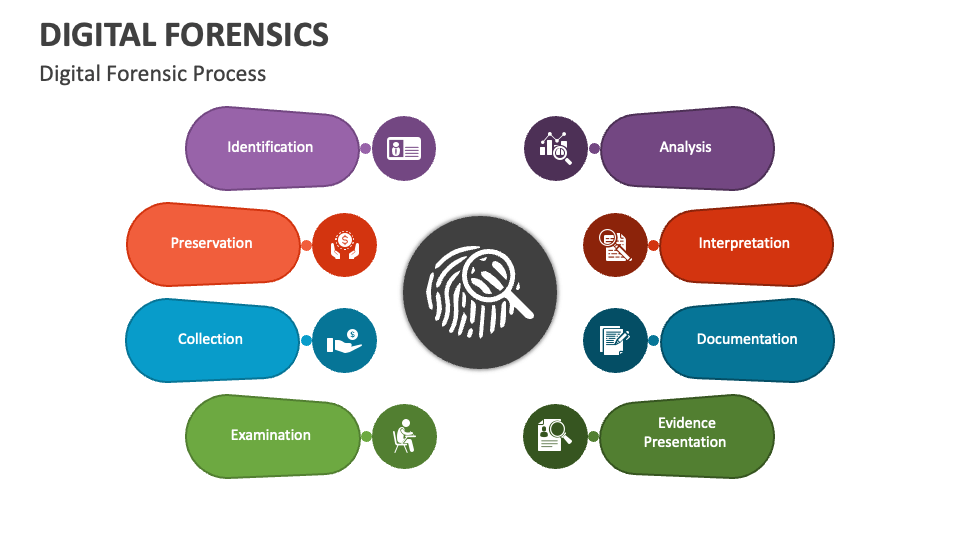
\includegraphics[width=0.9\textwidth]{img/digital-forensics-process.png}
    \caption{Dijital Adli Bilişim Sürecinin Temel Aşamaları ve Metodolojisi}
    \label{fig:digital-forensics-process}
\end{figure}

Adli bilişim, dijital ortamlarda işlenen suçları aydınlatmak için elektronik cihazlardan delil toplama, analiz etme ve hukuki raporlama sürecidir. Bir olay meydana gelmeden önce adli bilişim hazırlığının yapılması, müdahale süresini ve maliyetini azaltır. Bu hazırlık, olay müdahale planına adli bilişim süreçlerinin entegre edilmesini, personelin gerekli eğitimleri almasını ve yazma engelleyiciler, adli bilişim yazılımları (Autopsy, FTK Imager) gibi gerekli araçların hazır bulundurulmasını içerir.

\subsection{Delil Elde Etme: Canlı Sistem ve Post-mortem Analiz}

\begin{itemize}
    \item \textbf{Canlı Sistem Analizi (Live Forensics):} Bir sistem çalışırken, sistem kapandığında kaybolacak olan geçici (volatile) verilerin (bellek içeriği, çalışan süreçler, ağ bağlantıları) toplanmasıdır. Bu veriler, saldırganın sisteme nasıl sızdığına ve ne tür işlemler yaptığına dair kritik ipuçları sağlar.
    \item \textbf{Post-mortem Analiz (Post-mortem Forensics):} Sistem kapalıyken, kalıcı veri depolama birimlerinin (sabit disk, USB bellek) incelenmesidir. Bu işlem, bir delil diskinin bit-bit kopyasının (imajının) alınmasıyla gerçekleştirilir ve bu imaj üzerinde analiz yapılır.
\end{itemize}

\subsection{Bilgisayar Adli Bilişimi: Windows, Linux ve macOS İncelemesi}

Her işletim sisteminin kendine özgü yapısı, adli inceleme yöntemlerini de farklılaştırır.

\begin{itemize}
    \item \textbf{Windows:} Kayıt defteri (Registry) ve merkezi log yönetimi sayesinde analiz daha çok bu verilere odaklanır. Kayıt defteri, kullanıcı aktiviteleri (çalıştırılan programlar, dosya geçmişi) ve sistem yapılandırmaları hakkında zengin bilgi içerir.
    \item \textbf{Pratik Komut Örnekleri (PowerShell):}
    \begin{verbatim}
Get-EventLog -LogName Security -Newest 100
Get-ItemProperty -Path "HKCU:\Software\Microsoft\Windows\CurrentVersion\Run"
    \end{verbatim}
    \item \textbf{Linux:} Dağıtık günlükleme sistemi ve metin tabanlı yapılandırma dosyaları, daha çok manüel incelemeyi gerektirir.
    \item \textbf{Pratik Komut Örnekleri:}
    \begin{verbatim}
cat /var/log/auth.log | grep "Failed password"
find / -name "backdoor.sh"
    \end{verbatim}
\end{itemize}

\subsection{Ağ Adli Bilişimi ve Trafik Analizi}

Ağ adli bilişimi, bir siber saldırının izini sürmek, saldırı vektörünü belirlemek ve zararlı aktiviteyi ortaya çıkarmak için ağ trafiğini analiz etmeye odaklanır. Trafik, paket yakalama dosyaları (\texttt{.pcap}) halinde kaydedilebilir ve daha sonra incelenebilir.

\begin{itemize}
    \item \textbf{Araçlar:}
    \begin{itemize}
        \item \textbf{Wireshark:} Ağ trafiğini yakalayan, analiz eden ve protokolleri ayrıştıran en yaygın araçlardan biridir.
        \item \textbf{Snort:} Ağ Saldırı Tespit Sistemi (NIDS) olarak çalışarak önceden tanımlanmış kurallara uyan şüpheli paketler için alarm üretir.
    \end{itemize}
\end{itemize}
\textbf{Pratik Senaryo - Wireshark Analizi:}
Bir şüphelinin web sitesine yaptığı kullanıcı adı ve parola girişini incelemek için Wireshark kullanılabilir.
\begin{enumerate}
    \item \textbf{Yakalama:} Wireshark ile ağ arayüzü seçilerek paket yakalama başlatılır.
    \item \textbf{Filtreleme:} Yakalama tamamlandıktan sonra, trafiği daraltmak için \texttt{http.request.method == "POST"} gibi filtreler uygulanır.
    \item \textbf{Paket İncelemesi:} İlgili pakete tıklanarak TCP akışı takip edilir ve bu sayede oturum açma formuna girilen kullanıcı adı ve parola gibi hassas bilgiler incelenir.
\end{enumerate}

\subsection{Mobil Cihaz Adli Bilişimi ve Bulut Adli Bilişimi Zorlukları}

Bu alanlar, adli bilişimin en zorlu alanlarından biridir. Mobil cihazların cihaz çeşitliliği, işletim sistemi farklılıkları ve güçlü şifreleme mekanizmaları, delil elde etmeyi karmaşık hale getirir. Bulut adli bilişimi ise verilerin coğrafi olarak dağıtık olması, yasal yetki alanlarının belirlenmesi ve delilin mülkiyeti gibi sorunları beraberinde getirir.

\begin{itemize}
    \item \textbf{Pratik Yönergeler - Mobil Cihaz Delil Toplama:}
    \begin{enumerate}
        \item \textbf{İzolasyon:} Cihaz, uzaktan silme (remote wipe) veya veri manipülasyonu tehdidine karşı Faraday çantası gibi ekipmanlarla ağdan fiziksel olarak izole edilir.
        \item \textbf{Delil Elde Etme:} Cellebrite UFED veya Oxygen Forensic Detective gibi özel araçlarla cihazın fiziksel veya mantıksal imajı alınır.
    \end{enumerate}
\end{itemize}
Bu alandaki adli bilişim uzmanları, suçluların kullandığı teknolojinin gerisinde kalmamak için sürekli öğrenme ve araç kitlerini güncelleme baskısı altındadır. Mobil ve bulut teknolojilerindeki hızlı gelişmeler, geleneksel adli bilişim metodolojilerinin bu yeni dinamiklere adapte edilmesi gerektiğini göstermektedir.

\section{Uzmanlık Gerektiren Adli Bilişim ve İleri Düzey Analiz}

\subsection{Bellek Adli Bilişimi ve Uçucu Veri Analizi}

Bellek (RAM), bir sistem çalışırken oluşan ve sistem kapatıldığında kaybolan uçucu verileri (işlem parolaları, çalışan süreçler, ağ bağlantıları) içerir. Bu veriler, saldırının kapsamını ve amacını belirlemek için son derece değerli kanıtlar barındırır.

\begin{itemize}
    \item \textbf{Araçlar ve Teknikler:} \textbf{Volatility Framework} gibi bellek analizi araçları, RAM dökümünden bu uçucu verileri çıkarmak için kullanılır.
    \item \textbf{Pratik Yönergeler - Volatility ile Analiz:}
    \begin{enumerate}
        \item \textbf{Bellek Dökümü Alma:} Linux'ta \texttt{dd} komutu veya Windows için geliştirilmiş özel araçlar kullanılarak sistemin belleğinin ham kopyası (dökümü) alınır.
        \item \textbf{Analiz:} Volatility, bu döküm dosyası üzerinde bir dizi komut çalıştırarak analiz yapar:
        \begin{itemize}
            \item \texttt{python3 vol.py -f \textless{}filename\textgreater{} windows.pslist}: Çalışan tüm süreçleri ve ilişkili PID'lerini listeler. Birçok kötü amaçlı yazılım, gizli süreçler oluşturur ve bunlar bu listelerde tespit edilebilir.
            \item \texttt{python3 vol.py -f \textless{}filename\textgreater{} windows.netscan}: Bellek dökümü anındaki tüm ağ bağlantılarını, ilişkili süreçleri ve port bilgilerini listeler. Bu komut, bir komuta-kontrol (C2) sunucusuyla olan iletişimi ortaya çıkarabilir.
        \end{itemize}
    \end{enumerate}
\end{itemize}

\subsection{Veritabanı Adli Bilişimi ve Uygulama Log Analizi}

Veritabanları ve uygulamalar, kullanıcı aktiviteleri, hatalar ve kritik işlemler hakkında detaylı kayıtlar (loglar) tutar. Bu loglar, siber saldırıların tespiti, saldırganın hareketlerinin izlenmesi ve adli süreçlerde delil olarak kullanılması açısından hayati öneme sahiptir.

\begin{itemize}
    \item \textbf{Veritabanı Logları (SQL Server Örneği):}
    \begin{itemize}
        \item SQL Server, tüm işlemleri bir işlem günlüğünde (\texttt{.ldf} dosyası) kaydeder.
        \item Adli amaçlar için, \texttt{fn\_dblog()} gibi belgelenmemiş fonksiyonlar, aktif işlem günlüğünü sorgulamaya ve "kimin ne zaman, hangi veriyi değiştirdiği" gibi sorulara yanıt bulmaya olanak tanır.
    \end{itemize}
    \item \textbf{Uygulama Logları:}
    \begin{itemize}
        \item \textbf{Linux Ortamında:} \texttt{grep}, \texttt{awk} ve \texttt{sed} gibi komut satırı araçları, \texttt{syslog} veya \texttt{auth.log} gibi log dosyalarını manüel olarak incelemek için kullanılır.
        \item \textbf{Büyük Ölçekli Sistemlerde:} Logların merkezi olarak toplanması, işlenmesi ve görselleştirilmesi için Elasticsearch, Logstash, Kibana (ELK Stack) gibi kurumsal çözümler kullanılır.
    \end{itemize}
\end{itemize}

\subsection{Endüstriyel Kontrol Sistemi (ICS/SCADA) Adli Bilişimi}

ICS ve SCADA sistemleri, imalat, enerji ve su arıtma gibi kritik endüstriyel süreçleri yöneten sistemlerdir. Bu sistemler, eski teknolojiler, fiziksel etki potansiyeli ve özel ağ protokolleri nedeniyle benzersiz güvenlik ve adli bilişim zorluklarına sahiptir.

\begin{itemize}
    \item \textbf{Adli Bilişim Yaklaşımı:}
    \begin{itemize}
        \item \textbf{Ağ Segmentasyonu:} Saldırının operasyonel teknoloji (OT) ağından bilgi teknolojileri (IT) ağına yayılmasını önlemek için iki ağ fiziksel veya mantıksal olarak ayrılmalıdır.
        \item \textbf{Protokol Analizi:} Modbus, DNP3 gibi endüstriyel protokollere yönelik uzmanlık gerektiren paket analizi yapılır. Bu, saldırganın fiziksel süreçleri manipüle etmeye yönelik komutlarını ortaya çıkarabilir.
        \item \textbf{Sistem Log Analizi:} SCADA master ünitesindeki ve İnsan-Makine Arayüzü (HMI) cihazlarındaki loglar, saldırganın eylemlerini yeniden kurgulamak için incelenir.
    \end{itemize}
\end{itemize}

\subsection{Sanal Makine ve Konteyner Adli Bilişimi}

Sanallaştırma teknolojileri, adli bilişim süreçlerini karmaşıklaştırır.

\begin{itemize}
    \item \textbf{Sanal Makineler (VM):} Bir fiziksel makinenin dijital kopyasıdır ve kendi işletim sistemine sahiptir. VM üzerinde adli bilişim, fiziksel bir makinedekiyle benzer adımlar içerir, ancak analiz sanal disk imajları (\texttt{.vmdk}, \texttt{.vdi}) üzerinde yapılır.
    \item \textbf{Konteynerler (Docker):} İşletim sistemini sanallaştıran ve uygulamayı platformdan bağımsız çalıştıran hafif ortamlardır. Konteynerler geçici ve dinamik olduğu için adli incelemesi zordur. Şüpheli bir konteyner tespit edildiğinde, \texttt{docker commit} komutuyla mevcut durumu yeni bir imaj olarak kaydedilebilir ve bu imaj üzerinde dosya sistemi, bellek ve log analizi yapılabilir.
\end{itemize}

\subsection{Kripto Para ve Blockchain Adli Bilişimi}

Kripto paralar, merkeziyetsiz bir defter teknolojisi olan blockchain üzerinde çalışır. Bu teknoloji, kullanıcıları takma adlar (pseudonymous) kullanarak anonimleştirdiği için finansal suç soruşturmaları için bir zorluk oluşturur. Ancak, blockchain'in değişmez bir kayıt defteri olması, bir kez kaydedilen işlemin manipüle edilememesi anlamına gelir ve bu durum, suçla ilgili kanıtın güvenli bir şekilde saklanmasını sağlar. Adli bilişim uzmanları, kripto para birimlerine ait işlem kayıtlarını takip ederek para akışını izlemeye ve bu akışları gerçek dünya kimlikleriyle ilişkilendirmeye çalışır.

\section{Olay Sonrası Faaliyetler ve Kazanılan Dersler}

\subsection{Olay Dökümantasyonu ve Raporlama Gereksinimleri}

Olay müdahalesinin her aşaması, gelecekteki analizler ve hukuki süreçler için detaylı bir şekilde belgelenmelidir. Olay sonrası rapor (post-mortem), organizasyonun süreç iyileştirmesi için temel bir kaynaktır ve olayın "kim, ne, nerede, ne zaman, neden ve nasıl" sorularına yanıt vermelidir.

\begin{itemize}
    \item \textbf{Olay Sonrası Rapor Şablonu}
    \begin{tabular}{|l|l|l|}
    \hline
    \textbf{Bölüm} & \textbf{İçerik} & \textbf{Açıklama} \\
    \hline
    \textbf{Yönetici Özeti} & Olayın kısa özeti ve iş üzerindeki etkisi. & Olayın mahiyetine ve sonuçlarına ilişkin üst düzey özet. \\
    \hline
    \textbf{Olay Zaman Çizelgesi} & Olayın kronolojik olarak sıralanmış akışı. & İlk tespitten kurtarmaya kadar her eylemin zaman damgasıyla kaydı. \\
    \hline
    \textbf{Kök Neden Analizi} & Olayın temelinde yatan zafiyetler ve nedenler. & Saldırıya olanak sağlayan sistemsel, teknolojik ve operasyonel açıkların analizi. \\
    \hline
    \textbf{Alınan Aksiyonlar} & Sınırlama, yok etme ve kurtarma aşamalarında yapılanlar. & Hangi sistemlerin izole edildiği, hangi zararlı yazılımların kaldırıldığı, verilerin nasıl geri yüklendiği. \\
    \hline
    \textbf{Kazanılan Dersler ve Öneriler} & Gelecekte benzer olayların önlenmesi için iyileştirme önerileri. & Süreç, politika, teknoloji veya personel farkındalığına yönelik iyileştirme tavsiyeleri. \\
    \hline
    \end{tabular}
\end{itemize}

\subsection{Kazanılan Dersler Analizi ve Süreç İyileştirme}

Olaydan çıkarılan dersler, organizasyonel hafızayı güçlendirir ve aynı hataların tekrarlanmasını önler. Bu süreç, sürekli iyileştirme için bir geri bildirim döngüsü sağlar ve dört temel adımdan oluşur:

\begin{enumerate}
    \item \textbf{Belirleme:} Olaydan elde edilecek önemli kazanımların ve başarıların belirlenmesi.
    \item \textbf{Belgeleme:} Kazanılan derslerin, ilgili herkesin katkıda bulunabileceği bir formatta kaydedilmesi.
    \item \textbf{Analiz Etme:} Elde edilen verilerin incelenerek anlamlı sonuçlar çıkarılması.
    \item \textbf{Saklama:} Raporların, ekiplerin kolayca erişebileceği ortak bir dijital platformda arşivlenmesi.
\end{enumerate}

\subsection{Olaylardan Tehdit İstihbaratı Geliştirme}

Bir siber saldırı, organizasyon için değerli bir tehdit istihbaratı (CTI) kaynağıdır. CTI, ham veriyi (ör. zararlı IP adresleri) işleyerek anlamlı ve eyleme dönüştürülebilir bilgilere dönüştürme sürecidir.

\begin{itemize}
    \item \textbf{İki Önemli Kavram:}
    \begin{itemize}
        \item \textbf{Tehlike Göstergeleri (IOCs):} Kötü amaçlı IP adresleri, dosya hash'leri veya zararlı URL'ler gibi somut, teknik verilerdir. IOC'ler taktiksel düzeyde savunma için kullanılır.
        \item \textbf{Taktik, Teknik ve Prosedürler (TTPs):} Saldırganların amaçlarına ulaşmak için kullandığı yöntemlerdir. TTP'ler, IOC'lere göre daha kalıcıdır ve operasyonel düzeyde savunma için kritik öneme sahiptir.
    \end{itemize}
\end{itemize}
\textbf{İstihbarat Üretimi:}
Bir oltalama saldırısı sonrası tespit edilen zararlı dosya hash'i ve komuta-kontrol sunucusu IP adresi gibi IOC'ler toplanır. Bu veriler, saldırganın kullandığı genel yöntemlerle (ör. belirli bir zararlı yazılım ailesi) ilişkilendirilerek istihbarat haline getirilir ve gelecekteki saldırılara karşı otomatik koruma sağlamak için SIEM ve EDR sistemlerine entegre edilir.

\subsection{Eğitim ve Farkındalık Programı Güncellemeleri}

Bir siber saldırıdan elde edilen dersler, çalışan farkındalık eğitimlerini ve güvenlik prosedürlerini güncellemek için kullanılmalıdır. Olay sonrası yapılan analizler, çalışanların zafiyetli davranışlarını (ör. oltalama e-postalarına tıklama) ortaya çıkarır. Bu geri bildirimler, eğitim materyallerine dahil edilerek simülasyon bazlı testlerle çalışanların farkındalığı artırılır. Siber güvenlik eğitimlerinin de tıpkı diğer eğitim programları gibi, çağın gereklerine göre sürekli revize edilmesi, bu alanda durağanlığın mümkün olmadığının bir göstergesidir.

\subsection{Hukuki Süreç Desteği ve Uzman Tanık İfadeleri}

Siber güvenlik uzmanları, bir adli soruşturma veya mahkeme sürecinde "uzman tanık" olarak görev alabilirler. Hazırladıkları bilimsel mütalaalar, hukuka uygun, somut ve bilimsel verilere dayanmalıdır. Uzman, bulgularını ve vardığı sonuçları mahkemede net, anlaşılır ve basit bir dille açıklamalıdır. Uzmanın sunduğu rapor, hâkimin maddi gerçeği aydınlatmasına ve delilleri doğru yorumlamasına yardımcı olan bir araç olarak kullanılır. Bu durum, teknik uzmanlığın nihayetinde hukuki bir amaca hizmet ettiğini ve uzmanların raporlama ile iletişim becerilerinin de teknik yetkinlikleri kadar kritik olduğunu ortaya koymaktadır.